% # -*- coding: utf-8 -*-
%\section{Design and Implementation} \label{section:approach}
%\section{Design of vkTracer} \label{section:approach}
\section{Design} \label{section:approach}

%\subsection{Design Concept} \label{subsection:design}
% \subsection{Concept} \label{subsection:design}
\subsection{Requirement} \label{subsection:design}
% 提案するセキュリティ機構の設計においては,カーネルにおいて,指定したカーネル
% データへの書込み制限を指定するため,次の要件を満たすことを目指した.

% 提案するセキュリティ機構では,システムコール毎に動作中のカーネルにおいて保護対
% 象カーネルデータに対して読書き制限を指定するため,設計として次の要件を満たすこ
% とを目指した.
% This study 
% To manage write restrictions on specified kernel data in the kernel, we designed
To manage write restrictions on specified kernel data, 
% we designed the KDPM to satisfy the following requirement: 
% we considered 
the KDPM should satisfy the following requirement: 
% in order to manage write restrictions on specified kernel data in the kernel.

% User processes rely on kernel features to control system resources and hardware
% (i.e., memory, file system, and network). These kernel features are constructed
% from a set of kernel codes, and system calls are used instead of user processes
% to invoke kernel codes at the kernel layer.  
% %
% This study designed vkTracer to achieve the following requirements for tracking
% the invocation of vulnerable kernel codes.

\begin{figure*}[tb]
  \hspace{10.0ex}
  % \begin{center}
  % \centering
  % 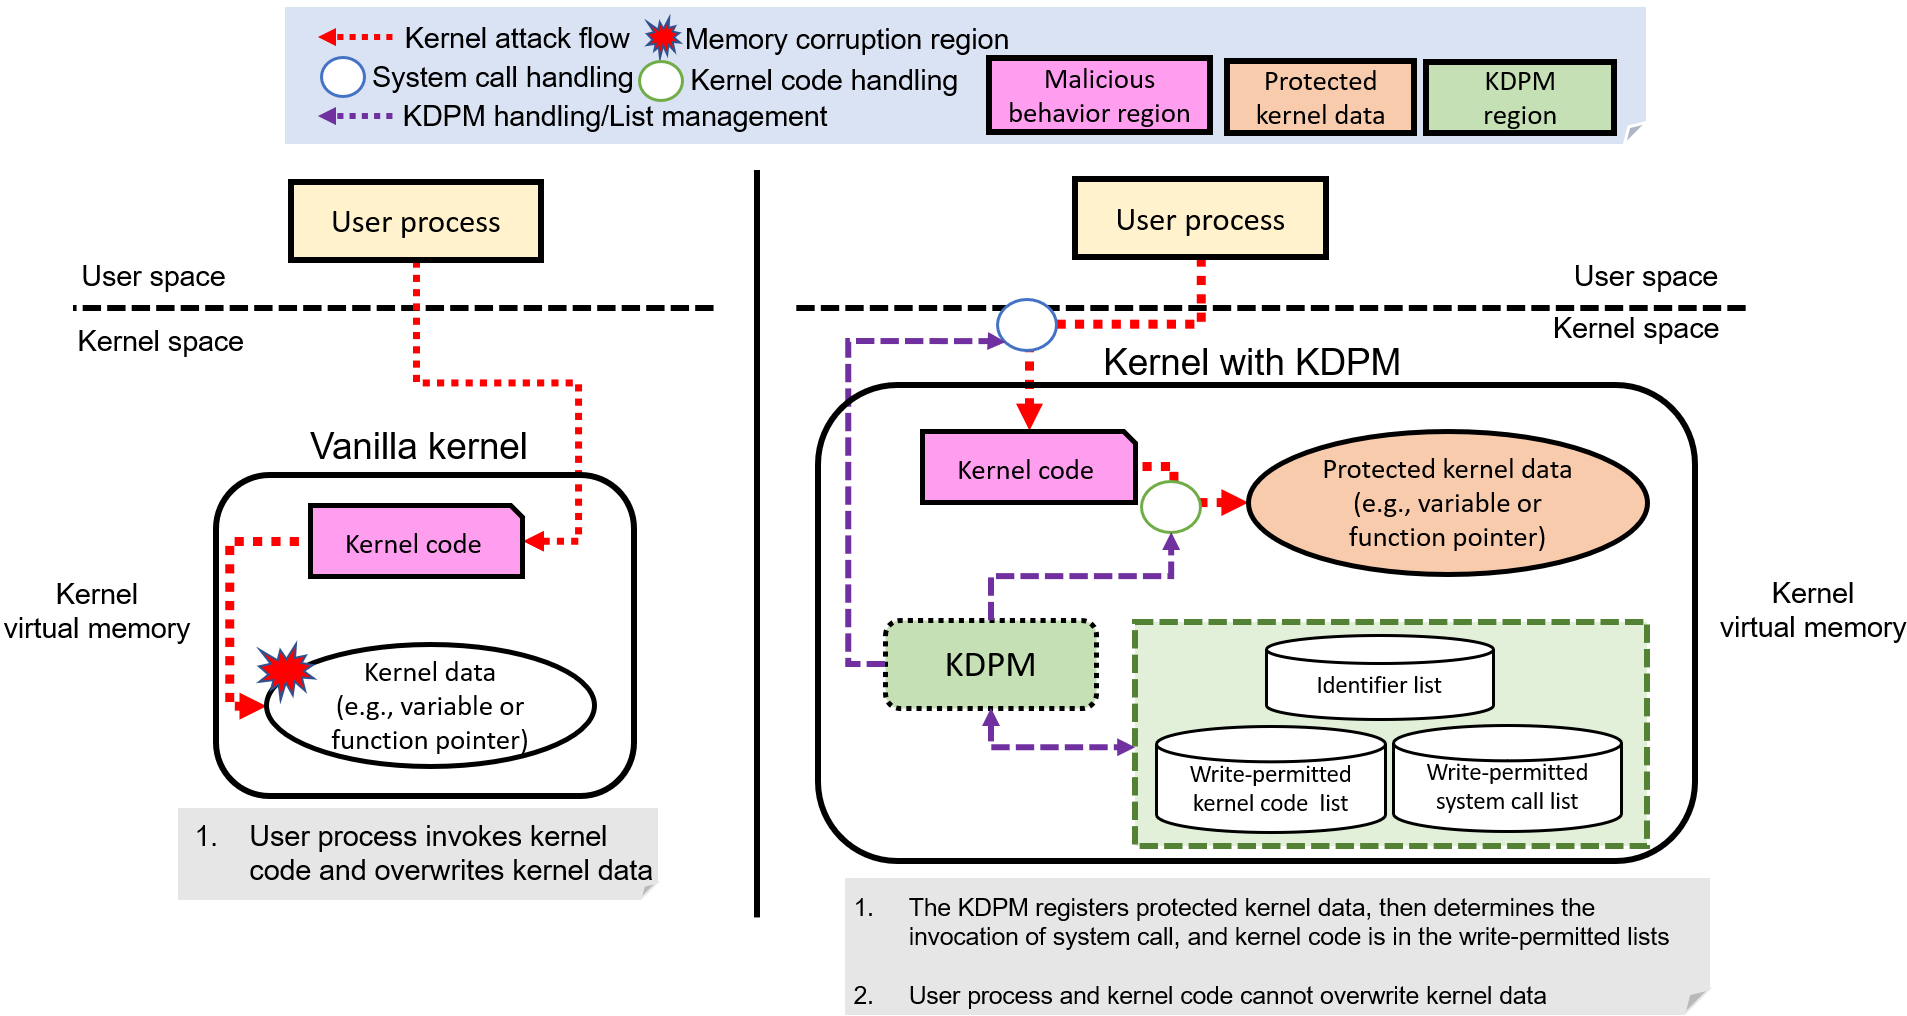
\includegraphics[bb=0 0 1587 852, scale=.280]{./imgs/003_screenshot_2021-07-27_19.37.39.png}
  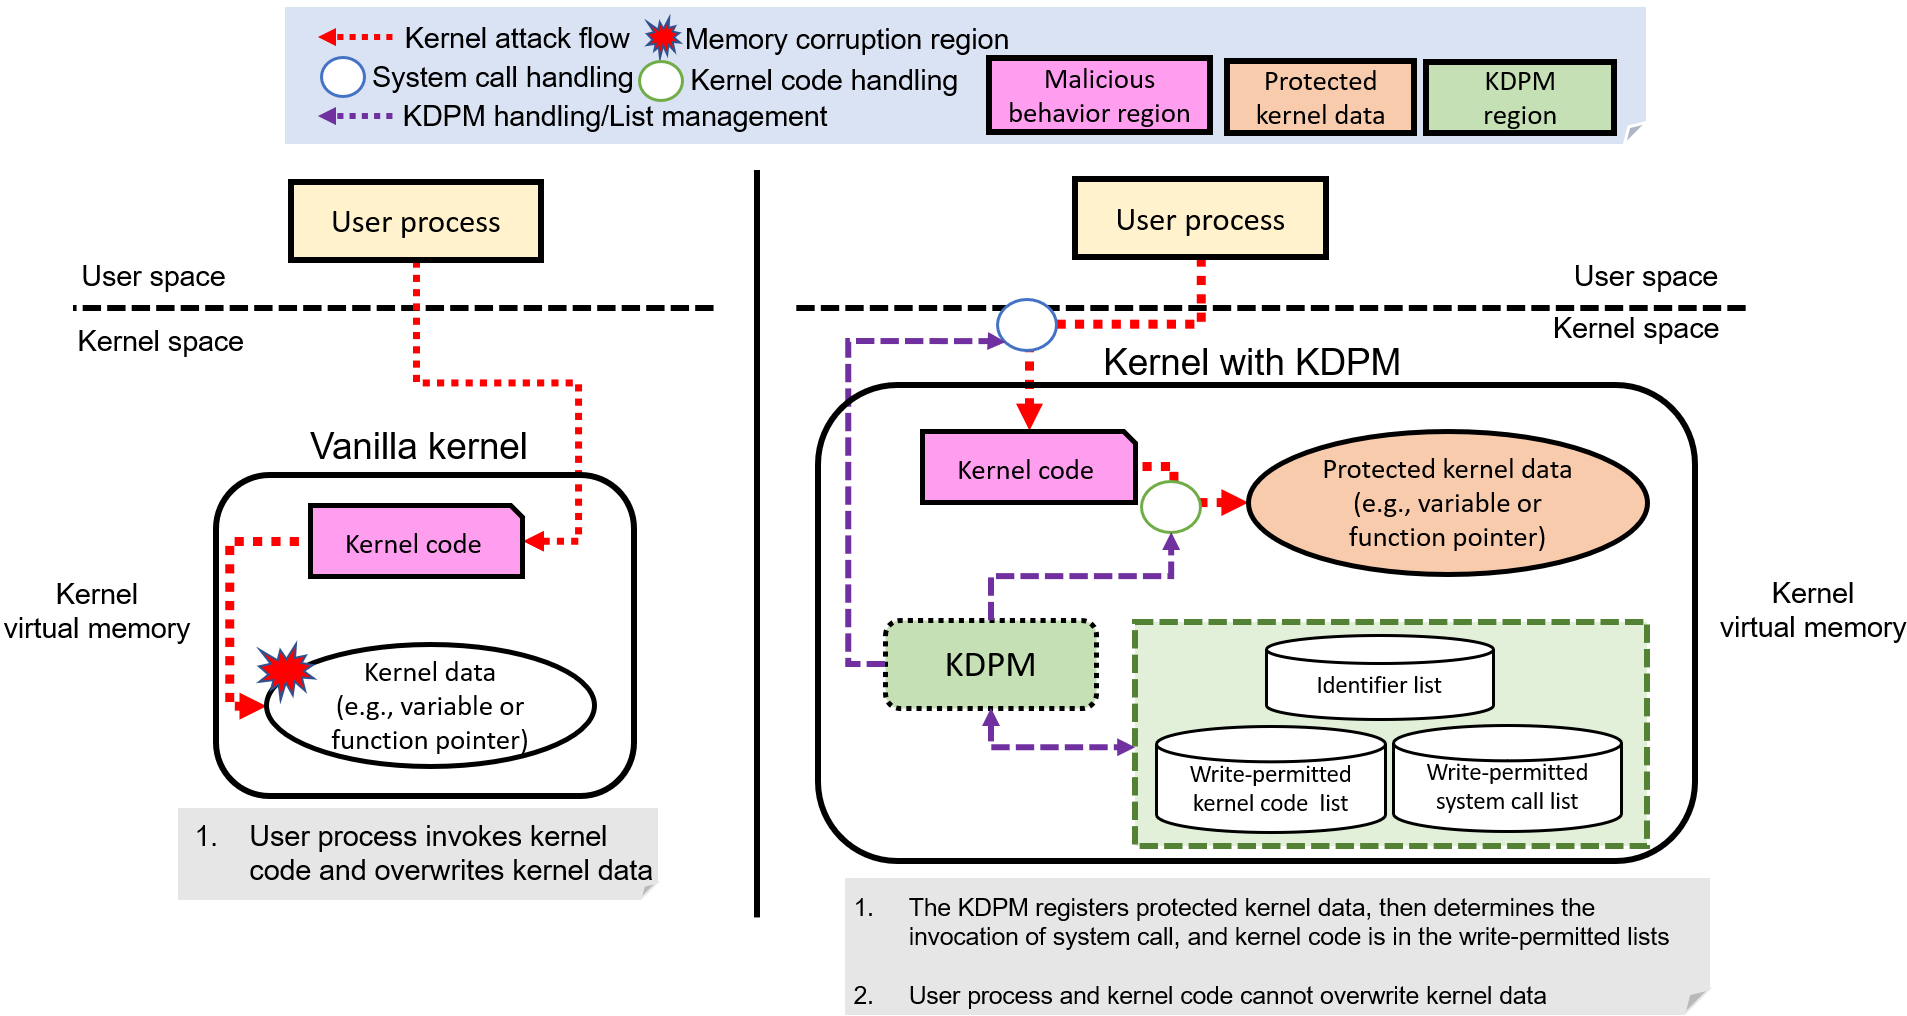
\includegraphics[bb=0 0 1430 762, scale=.320]{./imgs/003_screenshot_2021-07-27_19.37.39.png}
  % \end{center}
% \vspace{-1.5ex}      
  \caption{
    %
    %提案するセキュリティ機構の設計概要図
    Design overview of the KDPM
    %
  }
% \vspace{-0.5ex}      
% \vspace{-3.5ex}
 \label{fig:design_overview}
\end{figure*}


\begin{itemize}%\itemsep=-1.0ex \parskip=1.0ex
  % カーネル脆弱性を利用したカーネルデータの改ざんによる特権昇格,ならびにセキュ
  % リティ機能の無効化攻撃を緩和する.
  % %
  % カーネルデータに対する書込み制限の管理として,保護対象に指定したカーネルデー  
  % タ毎に書込み制限制御を特定のシステムコール単位,ならびにカーネルコード単位で
  % 処理可能とする.
  % %
  % 書込みを許可されたシステムコールに関するカーネルコード,ならびにカーネルコー
  % ドの実行中においてのみ保護対象に指定したカーネルデータへの書込みを可能とす
  % る.
\item {\bf Requirement}: Prevent privilege escalation and defeat of security mechanisms
 by illegally modifying kernel data via kernel vulnerabilities.
  %
  The kernel must control the write restrictions of kernel data for specific
  system calls and kernel codes on the running kernel.
  %
  The kernel data can be written only %during the invocation of 
  when system calls are invoked and the authorized kernel codes are executed.
% disablement attacks   
  % can be controlled 
    % for each kernel data specified as the target of  protection.
  % kernel code related to 
  %  to be written.

  % 攻撃を行うユーザプロセスによるカーネル脆弱性を利用したカーネルデータ
  % の改ざん(例,特権奪取攻撃)を想定し,保護対象カーネルデータの読書き
  % 制限を設定可能とする.
  % %
  % 動作中のカーネルにおける読書き制限の管理として,書込み制限の制御は
  % システムコール単位で処理する.
  % %
  % 読書き制限の切替えはシステムコール発行時に行い,書込みを許可され
  % るシステムコールの実行中においてのみ保護対象カーネルデータへの書込み
  % 制限を無効可能とする.


% \item Requirement 1 (R1): Trace the invocation of a
%   vulnerable kernel code that leads to memory corruption or DoS.
%   %
%   The tracing feature must trap the behavior of the adversary's user process and
%   kernel while the vulnerable kernel codes are invoked on the running kernel.

% \item Requirement 2 (R2): Identify the vulnerable kernel
%   code. 
%   %
%   The profile of the kernel vulnerability must contain the list of virtual address
%   ranges and function names. These are identified from the list of invoked
%   vulnerable kernel codes.
\end{itemize}

% \subsection{Challenges}

% vkTracer fulfills the requirements for identification and hooking the
% invocation of vulnerable kernel codes using a combination of tracing
% and restriction of the kernels.
% The challenges faced during the tracing and identification of vulnerable kernel codes
% are as follows:

% \begin{itemize}%\itemsep=-1.0ex \parskip=1.0ex
%   %
%   \item R1 raises the question of how to trace running kernel behavior during
%   an adversary's user process execution.
%   %
%   The attaching of the kernel is difficult from the user process, but kernel
%   features should introduce the hooking of all kernel code invocations.
%   %
%   This mechanism allows the tracing of entry points that can be registered to the
%   running kernel from the user process.  %when the adversary's

%   \item R2 raises the question of how to analyze the kernel structure with
%   the vulnerable kernel code invocation list.
%   %
%   The kernel should support symbol information for the running kernel and should
%   embed kernel component information into the static kernel image at the kernel
%   compilation time.
%   %
%   This mechanism allows an analysis of the relationship among the function
%   name, virtual address, and the invocated vulnerable kernel code for the profile
%   generation.

% \end{itemize}

\subsection{Design Overview}

KDPM fulfills the requirement for kernel data protection from the invocation of
vulnerable kernel codes. 
%
Figure \ref{fig:design_overview} outlines the design overview of 
% It is 
%
KDPM introduces the protected kernel data, identifier list, the
write-permitted system call list and write-permitted kernel code list.

%
% that stores the kernel data 
%the management of linking the identifier to the
KDPM manages the linking of the identifier that indicates the relationship between
the protected kernel data, write-permitted system call, and write-permitted kernel
code.
%
KDPM statically registers protected kernel data, identifiers of protected kernel
data, write-permitted system call, and write-permitted kernel code lists at the
source code. After that, KDPM dynamically controls the write restriction of
kernel data using identifier at the invocation of system call or kernel code for
the running kernel.

\subsection{Approach}
% 提案するセキュリティ機構として,要件を満たす設計概要を図
% \ref{fig:design_overview}に示す.
% %
% 提案するセキュリティ機構では,保護対象カーネルデータの書込み制限の制御に用いるために,
% 保護対象として指定するカーネルデータ(例,変数値,
% および関数ポインタ),ならびに識別子を設ける.
% そして,識別子をシステムコール,およびカーネルコードと紐付けて制御の管理を行う.

% 提案するセキュリティ機構の設計概要を\figref{fig:design_overview}に示す.
% 要件を満たすため提案するセキュリティ機構では,保護対象カーネルデータ
% (例,権限情報)を予め指定し,識別子を設けて管理する.また,システムコー
% ルと紐付け,保護対象カーネルデータの読書き制限を管理する.
%The KDPM supports the kernel data as protected kernel data (e.g., variable or
The KDPM supports specific kernel data as protected kernel data (e.g., variable
or function pointer) and the identifier to handle the write restrictions that
manages the write-permitted system calls and write-permitted kernel code.
%satisfy the aforementioned requirement.
%
% The proposed security mechanism defines and manages the following two types:
% system calls and kernel code.
%
% The following protected kernel data and identifier for restriction must be
% fulfilled:

% \subsubsection{保護対象カーネルデータ}
\subsubsection{Protected Kernel Data:}

The following are the definitions of protected kernel data and identifiers:
% to be managed by the proposed security
% mechanism 


% 提案するセキュリティ機構において管理する保護対象カーネルデータおよび識別子は次の
% 通りとする.

\begin{itemize}
% \begin{itemize}[topsep=0pt]%\topsep=-1.0ex \itemsep=-1.0ex \parskip=1.0ex%\topsep=-1.0ex \itemsep=-1.0ex \parskip=1.0ex
  
% \item 保護対象カーネルデータ:ユーザプロセスのカーネルデータ(例.権限情報),お
% よびカーネルにおけるセキュリティ機能において利用されるカーネルデータ(例.関数ポ
% インタ)
\item Protected kernel data: The kernel data of the user process (e.g.,
privileged information) and security mechanisms (e.g., the function pointer
and access policy).
% Kernel data of the user process (e.g., privileged information) and the kernel data of security mechanism (e.g., function pointer and access policy).
% in the kernel (e.g. (function pointer).

\item Identifier: The identifier is used to set the write restrictions of the
protected kernel data. For controlling the write restriction, the identifier is
associated with the protected kernel data, write-permitted system call, and
write-permitted kernel code.

% \item 識別子:保護対象カーネルデータの読書き制限を設定するために用いる識別子.書
%   込み制限制御のため,識別子に対し,保護対象カーネルデータ,および,書込み許可シ
%   ステムコール,書込み許可カーネルコードの紐付けを行う.
%   %書込み許可システムコール,書込み許可カーネルコードの紐付けを行う.
  
\end{itemize}


% 提案するセキュリティ機構を備えたカーネルでは,起動時に保護対象カーネル
% データと対応する識別子のリストを予め設ける.
% %
% 動作中のカーネルにおいて,保護対象カーネルデータはユーザプロセス毎に生
% 成されることを想定し,ユーザプロセスの起動時にて,識別子との関連づけを
% 行い,同時に読書き制限を設定する.
The kernel with the KDPM provides a list of protected kernel data and
corresponding identifiers in advance at the time of booting.
%
Additionally, the kernel data for each user process generation is assumed to be
protected.

% At the startup of the user process, the identifier is associated with the kernel
% data to be protected, and the read restriction is set at the same time.

% 提案するセキュリティ機構では,カーネル内部において,保護対象カーネルデータ,識別
% 子のリストを予め設ける.

% 提案するセキュリティ機構における保護対象カーネルデータおよび識別子は次
% の通りである.

% %\begin{itemize}
% \vspace{-2.0ex}
% \begin{itemize}\topsep=-1.0ex \itemsep=-1.0ex \parskip=1.0ex
% \item 保護対象カーネルデータの識別子:読書き制限を設定するために用いる
%   カーネルデータ種別を示す識別子.識別子に対して読書き制限の紐付けと設
%   定を行う.
  
% \item 保護対象カーネルデータ:アプリケーションをユーザプロセスとして実
%   行する際,カーネルにおいて設定されるカーネルデータ.
  
% \end{itemize}
% \vspace{-2.0ex}




%To satisfy the challenge of vkTracer, the enhancement of the
%capability for the kernel.
% vkTracer addresses the aforementioned challenges by enhancing the capabilities of
% the kernel.
% %
% Figure \ref{fig:approach_overview} outlines how vkTracer
% generates a profile by tracing the invocation of a vulnerable kernel
% code from the PoC code.
% %
% The following approach provisions for tracing and restriction must be
% fulfilled:


%\vspace{-1.0ex}    
% %\begin{itemize}%\itemsep=-1.0ex \parskip=1.0ex
% \begin{itemize}%[topsep=0pt,leftmargin=0.5cm]%\itemsep=-0.5ex
% \item {\bf Vulnerable kernel code dynamic tracing and analysis}\\
% %{\bf Vulnerable kernel code dynamic tracing and analysis}\\
% %The capability of 
% vkTracer provides a mechanism for dynamic kernel tracing and for the analysis of an
% adversary's user process (e.g., execution of PoC codes) in the running kernel.
% %
% vkTracer traps the invocation of vulnerable kernel codes that is
% requested when the adversary's user process attempts to exploit a
% kernel vulnerability.
% %
% Furthermore, this mechanism utilizes the symbol and debugging information of the
% static kernel image during tracing. This mechanism ensures that vulnerable
% kernel code information (e.g., virtual address range and function name) is used
% to generate a profile of a specific kernel vulnerability.


% \end{itemize}
%\vspace{-1.0ex}



% \subsubsection{読書き制限の管理と操作}
\subsubsection{Handling of Write Restrictions:}
% % \subsubsection{読書き制限の管理と制御}

% 提案するセキュリティ機構において,保護対象カーネルデータへの読書き制限制御は特
% 定のシステムコール,およびカーネルコードにて行う.
% %
% 提案するセキュリティ機構では,次の2種類を定義し,管理する.書込み制限の制御
% は,システムコールの発行時,ならびにカーネルコード実行時において書込み制御機能
% を呼出すことで行う.
The KDPM handles the write restrictions of the protected
kernel data using specific system calls and kernel codes.
%
The KDPM defines and manages the following:

%\begin{itemize}[topsep=0pt]%\topsep=-1.0ex \itemsep=-1.0ex \parskip=1.0ex%\topsep=-1.0ex \itemsep=-1.0ex \parskip=1.0ex      
\begin{itemize}
% \item 書込み許可システムコール:保護対象カーネルデータの書込み権限を有するシス
%    テムコール.
\item Write-permitted system call: A system call has write permission for
the protected kernel data.

% \item 書込み許可カーネルコード:保護対象カーネルデータの書込み権限を
%   有するカーネルコード.
\item Write-permitted kernel code: The kernel code is authorized to write
to the protected kernel data. 
% The kernel code that has the following features.

\end{itemize}
% %\vspace{-2.0ex}

% %提案するセキュリティ機構における読書き制限制御は,システムコールおよび
% %タへの書込みを許可する.その後,システムコールおよびカーネルコードの実
% 提案するセキュリティ機構における書込み制限制御は,書込み許可システムコール発行
% 時,および書込み許可カーネルコード実行前に,識別子に基づき,保護対象カーネルデー
% タへの書込みを許可する.その後,システムコール終了時,およびカーネルコード実行後
% に保護対象カーネルデータへの書込みを制限する.

The KDPM disables write restrictions when a write-permitted system
call is issued or write-permitted kernel code is executed.
% at the time of issuing at the time of 
% invthe write control function at the 
%
%The write restriction control in the proposed security mechanism is performed
%when a write-allowed system call is issued and when write-allowed kernel code is
%executed. 
% The kernel data to be protected is controlled for write permission based on the
% specified identifier with system call or kernel code. 
At the end of the write-permitted system call or write-permitted kernel code
execution, the KDPM enables the write restriction to the protected kernel data.



% %
% 提案するセキュリティ機構では,識別子毎に書込み許可リストとして,書込み許可システ
% ムコール,および書込み許可カーネルコードのリストを管理し,書込み制限の管理制御に用
% いる.


% 提案するセキュリティ機構において,保護対象カーネルデータへの読書き制限
% はシステムコール単位で行う.
% %
% システムコールを次の2種類に分類して管理し,システムコールの発行毎に読
% 書き制限を操作することで取扱う.

% %\begin{itemize}
% \vspace{-2.0ex} 
% \begin{itemize}\topsep=-1.0ex \itemsep=-1.0ex \parskip=1.0ex      
% \item 権限変更許可システムコール:保護対象カーネルデータの書込み権限を
%   有するシステムコール.

% \item 通常システムコール:保護対象カーネルデータの書込み権限を有さない
%   システムコール.
% \end{itemize}
% \vspace{-2.0ex}

% 提案するセキュリティ機構を備えたカーネルでは,権限変更許可システムコー
% ルのリスト(以降,権限変更許可リスト)を管理する.動作中のカーネルにお
% いて,権限変更許可リストのシステムコール発行時に保護対象カーネルデータ
% の読書き権限を変更する.
% %権限情報 Protection key に基づく
% 権限変更許可システムコールの実行時のコンテキストでのみ,保護対象カーネ
% ルデータの書込み制限は無効化され,カーネルにおいて権限情報の変更が許可
% される.
% %
% 通常システムコールの実行時,保護対象カーネルデータへの書込み制限はカー
% ネルにおいて有効化され,書込みは制限される.


% \subsection{Profile of Vulnerable Kernel Codes}
% vkTracer traps all invocations of the kernel codes.
% %
% Figure \ref{fig:approach_overview} depicts an adversary's user
% process in the tracing environment.
% %
% vkTracer executes the PoC code when an adversary's user process
% invokes the vulnerable kernel code through the known kernel
% vulnerability on the running kernel.
% %
% vkTracer identifies the vulnerable kernel code and generates a
% profile of kernel vulnerability, and it is defined as follows:
% a profile of kernel vulnerability, as follows:


% %\subsection{Profile}
% \begin{itemize}%\itemsep=-1.0ex \parskip=1.0ex
% \item {\bf Profile}:
%   This profile consists of a list of the kernel code invocations,
%   virtual address range, and function name.
%   %
%   vkTracer automatically collects the invocations of the kernel code instigated by
%   the adversary's user process and then identifies the virtual
%   address range and function name of the vulnerable kernel code.
  
% \end{itemize}



% \subsection{Termination Condition} 
% %
% vkTracer defines the condition of tracing completion when the user
% process completes the attack scenario (in Section
% \ref{subsection:attack_scenario}).


% %
% After vkTracer finishes the trapping of the PoC code, % as the user process, 
% it starts to generate a profile of kernel vulnerability based on the necessary
% information from the tracing result.


%% Profile is the list of the invocations of kernel code,
  %% virtual address range, and function name.
  %% %
  %% vkTracer automatically collects the invocations of
  %% kernel code of adversary's user process, then identifies virtual
  %% address range and function name of vulnerable kernel code.

    %The tracing of KPRM collects a tracing result contains
    %the invocation of kernel code list after the PoC code as
    %adversary's user process that successes to exploit kernel
    %vulnerability on the running kernel.
    %to achieve the privilege escalation with memory corruption.
  
    %using the tracing
    %result of adversary's user process using dynamic and static kernel
    %information.
 % }

  %% PoC code is small set of attacking sequence that
  %% requires the invocation of vulnerable kernel code.
  
  %% the tracing of KPRM.
  %% to an adversary's user process. 

%% depicts the adversary's user
%% process on the tracing environment.
%% %
%% vkTracer identifies the vulnerable kernel code to generate a profile
%% of kernel vulnerability.
%
  %for identification of kernel vulnerability.
  %for the kernel attack surface reduline.
  %of kernel vulnerability.
  %kernel pages for the  adversary's user process.
  %
  %The left side of Figure \ref{fig:approach_overview} depicts the adversary's
  %user processes X on the tracing of KPRM.
%  }
%
%
%% \blueuline{ The restriction of KPRM adopts unmapping management from
%%   the kernel address space to handle the kernel page references for
%%   controlling the execution privilege and data access privilege on the
%%   restricted kernel page.
%%   %
%%   It achieves that The adversary's user process cannot invoke the vulnerable kernel
%%   code and access the kernel data on restricted pages.
%% }
%\subsubsection{プロファイル生成}
%% 要件を満たす設計として,図\ref{fig:approach_flow_overview}に提案手法の
%% 処理概要を示す.提案手法では,動作中のカーネルにおいて,ユーザプロセス
%% の実行に対応するカーネルコードの実行を追跡し,攻撃実行時,および攻撃未
%% 実行時のカーネルコードを呼出処理に応じて取得する.
%% %

%\reduline{

%% \subsection{Tracing and Identification Situations}
%% vkTracer generates a profile to manage vulnerable kernel code in the following situations.
%% \vspace{-1.0ex}
%% \begin{itemize}
%% \item {\bf Situation 1}:
%%   The kernel vulnerability is locally exploited by the adversary's
%%   user process.
  
%%   vkTracer traces the adversary's user process and running kernel.
  
%%   In this case, the adversary's user process directly invokes the
%%   vulnerable kernel code, then vkTracer collects all invocations of
%%   kernel code to generate the profile.
  
%% \item {\bf Situation 2}:
%%   The kernel vulnerability is remotely exploited by the adversary's
%%   user process.  
  
%%   vkTracer traces the adversary's user process and running kernel
  
%%     KPRM moves the vulnerable kernel code is on a restricted kernel page.
%%   The adversary's user process cannot access any restricted kernel page.
%%   If the adversary's user process attempts to execute the vulnerable
%%   kernel code, the kernel issues a page fault;
  
%%   KPRM does not allow execution of the vulnerable kernel code for the
%%   adversary's user process, which is killed after completion of the
%%   page fault handler.

%% \item {\bf Situation 3}:
%%   The profile contains the attack target kernel data.
  
%%   Although the vulnerable kernel code is on a normal kernel page, KPRM
%%   moves the attack target kernel data is on a restricted kernel page.
  
%%   If the adversary's user process executes the vulnerable kernel code
%%   that tries to override the target kernel data, the kernel issues a
%%   page fault;
  
%%   KPRM catches this page fault, and then kills the adversary's user
%%   process owing to access of the restricted kernel page.
  
%% \end{itemize}  


%\subsubsection{Profile Generation}
%


  %% vkTracer executes the PoC code as adversary's user
  %% process that invokes the vulnerable kernel code through the already
  %% known kernel vulnerability on the running kernel.
  %% %
  %% vkTracer defines a profile of kernel vulnerability as following.

%% プロファイルは,提案手法により収集したカーネル脆弱性に関するカーネルコー
%% ドと仮想アドレス範囲の組合せとする.
%\reduline{
%
  %for the restriction 
  %
  %The tracing of KPRM genarates a profile that contains
  %virutal address range and function name of vulnerable kernel
  %code.
%}
%% プロファイルの生成のため,カーネル脆弱性を利用したPoCコードを用いる.
%% カーネル脆弱性を利用した攻撃が成功する際のカーネルコードの一覧は,攻撃
%% 実行時の追跡結果と攻撃未実行時の追跡結果より取得する.



%% \begin{itemize}
%% \item 攻撃実行時:PoC コード実行時に攻撃が行われ,かつ
%%   攻撃が成功したと判定された場合に呼出されるカーネルコードの一覧.
  
%% \end{itemize}

%% %
%% カーネルへの攻撃に関与しない,ユーザプロセスの実行に必要とされる汎用的,
%% または一般的なカーネルコードの一覧を追跡結果として得るため,攻撃未実行
%% 時として,攻撃を行うプログラムコードを除外したPoCコードを実行する.
%% %
%% PoCコードのプログラムサイズが小規模である場合,攻撃未実行時のカーネル
%% コード一覧は攻撃実行時にも含まれると考えている.
%% %
%% 攻撃実行時のみに含まれるカーネルコードと仮想アドレス範囲の組合せをカー
%% ネル脆弱性を用いて攻撃が成功する際のカーネルコードの一覧として抽出し,
%% プロファイルとする.
%\label{subsubsection:tracing_condition}
%% 追跡対象のユーザプロセスを実行した際,\ref{subsection:design} 節で示し
%% た一連の処理により,カーネルにおいてユーザプロセスから呼び出されたカー
%% ネルコードが列挙され,最終的にカーネルコードに対応する仮想アドレス範囲
%% の一覧が得られる.カーネルへの攻撃に紐づくカーネルコードかの判断は,カー
%% ネル脆弱性を利用した攻撃の成功可否を判定して行う.
%% %攻撃の成功可否を判定することが必要である.
%\reduline{



%% \begin{itemize}\itemsep=-1.0ex \parskip=1.0ex

%% \item {\bf Privilege Escalation}:
%%   The adversary's user process forcibly modifies its credential
%%   information to the administrator privilege from the normal privilege.

%% \item {\bf DoS}: The adversary's user process forcibly suspend the
%%   running kernel after the exploiting of kernel vulnerability.  It is
%%   difficult to continue the tracing of user process and kernel,
%%   vkTracer writes the history of vulnerable kernel code invocation to
%%   the disk or send these to the remote server.

%% \end{itemize}


%vkTracer defines the condition of tracing completion when
%the user process completes the attacking scenario
%
%% After vkTracer finishes the trapping of the PoC code as the user
%% process, vkTracer starts to generate a profile of kernel vulnerability
%% from the necessary information of tracing result.

  %}% in \ref{subsection:attack_scenario}. }

%% 提案手法においては,カーネル脆弱性を介して攻撃可能なPoC コードを実行す
%% る際に,以下のカーネル脆弱性毎の攻撃成功可否基準に従い,攻撃の有効性を
%% 判定する.
%% %攻撃成功時には基づいてカーネル脆弱性および関連するカーネルコードを特定する.

%% %,カーネルコードの推測が可能だと考えているが,CVE,PoCコー
%% %ド,ならびにカーネルのソースコード修正履歴を参照しながら特定する必要が
%% %ある.

%% \begin{itemize}%\itemsep=-1.0ex \parskip=1.0ex

%% \item {\bf Privilege Escalation}:
%%   The adversary's user process forcibly modifies its credential
%%   information to the administrator privilege from the normal privilege.

%% \item {\bf DoS}: The adversary's user process forcibly suspend the
%%   running kernel after the exploing of kernel vulnerability.  It is
%%   difficult to continue the tracing of user process and kernel,
%%   vkTracer writes the history of vulnerable kernel code invocation to
%%   the disk or send these to the remote server.

%% \end{itemize}

%% \begin{itemize}
%% \item 特権奪取:攻撃を行うユーザプロセスの実行前後において,権限情報の
%%   通常ユーザから特権ユーザへの変化を攻撃成功とみなす.

%% \item DoS:攻撃を行うユーザプロセスの実行中にカーネルが停止した場合,
%%   攻撃成功とみなす.カーネルが停止する場合,カーネルコードの呼出し履歴
%%   の取得が困難となることから,永続性のある記録媒体へのカーネルコードの
%%   呼出毎の保存,またはリモートの計算機へのログ出力を行う.

%% \end{itemize}


%% カーネル脆弱性毎の攻撃成功可否基準を利用し,
%% %攻撃を行うユーザプロセスからの要求に伴い実行されたカーネルコードから
%% %カーネルコードとして,
%% 攻撃成功と判定された場合のみ,攻撃実行時におけるユーザプロセスからの要
%% 求に伴い実行されたカーネル脆弱性に関連するカーネルコードの一覧とする.


%% \subsection{Restriction Design}
%% %
%% \blueuline{
%%   The restriction of KPRM assignes vulnerable kernel code, the kernel
%%   code, and kernel data to the restricted kernel pages for the
%%   adversary's user process.
%%   %
%%   The right side of Figure \ref{fig:approach_overview} depicts the adversary's
%%   user processes X on the KPRM kernel.
%%   }
%% %
%% %
%% \blueuline{ The restrictio of KPRM adopts unmapping management from
%%   the kernel address space to handle the kernel page references for
%%   controlling the execution privilege and data access privilege on the
%%   restricted kernel page.
%%   %
%%   It achieves that The adversary's user process cannot invoke the vulnerable kernel
%%   code and access the kernel data on restricted pages.
%% }

%% \subsubsection{Kernel Page Types}

%% \blueuline{
%%   The restriction of KPRM provides two types of kernel page structures, the restricted kernel
%%   page list, and benign user process list for the kernel.
%% }

%% %\vspace{-1.0ex}    
%% \begin{itemize}%\itemsep=-1.0ex \parskip=1.0ex

%% \item {\bf Normal kernel page}:
%%   \blueuline{%Every user process and kernel task share normal pages.
%%     This is shared by every user process and kernel task.
%%     A normal page contains the kernel code and kernel data.}
%%   %This is shared by every user process and kernel task. It contains the kernel code and kernel data.

%% \item {\bf Restricted kernel page}:
%%   %
%%   \blueuline{
%%     %An adversary's user process has the assignment of restricted kernel pages.
%%     This is assigned to an adversary's user process.
%%     During kernel execution, the restriction of KPRM forcibly unmaps restricted kernel page references
%%     for an adversary's user process.
%%   }
    
%%     %KPRM unmaps restricted kernel page references during kernel execution.
%% \end{itemize}
%% %\vspace{-1.0ex}    

%% \blueuline{
%%   To create a restricted kernel page list,
%%   the restriction of KPRM can automatically calculate a valid page frame number
%%   from the virtual address of kernel code and kernel data.
%% }
%% %
%% \reduline{
%%   The virtual address of kernel code is induced from a profile of kernel vulnerability
%%   and target kernel data is statically implemented in the kernel.
%%   }
%% %
%% KPRM specifies restricted kernel pages when all the vulnerable kernel
%% code and kernel data are identified at the kernel booting.
%% %
%% Additionally, KPRM manages the restricted kernel page
%% list that stores and deletes a restricted kernel page.
%% %
%% \blueuline{
%%   The user process has the benign identifier flag for the management of the benign user process list
%%   %that manually contains benign user process identifiers
%%   to avoid the restricted kernel page management at the running kernel.
%% }

%% %% \subsection{排他ページの格納オブジェクトの対象}
%% \subsubsection{Restricted Kernel Page Object}

%% \blueuline{
%%   The restriction of KPRM provide a restricted kernel page that provide the assignments of
%%   the following kernel code and kernel data for security capability.
%%   %The restriction of KPRM supports the following kernel code and kernel data for protection
%% }

%% %\begin{enumerate}[leftmargin=2.4cm]%\itemsep=-1.0ex \parskip=1.0ex
%% %\vspace{-1.0ex}    
%% \begin{itemize}%\itemsep=-1.0ex \parskip=1.0ex
%% %\begin{itemize}

%% \item {\bf Kernel code}: It is a component of the kernel features 

%% \item {\bf Kernel data}: It is a variable of privilege information

%% \end{itemize}
%% %\vspace{-1.0ex}    
%% %\end{enumerate}

%% \blueuline{
%%   Specifically, KPRM assumes that kernel code is already known kernel vulnerability
%%   that is discovered or reported} in \cite{cvedetails},
%%   and kernel data are credential variables of
%%   the running user process.

%% %% Specifically, KPRM assumes that kernel code is already known, and that
%% %% the kernel vulnerability and kernel data are credential variables of
%% %% the running user process.


%% \subsubsection{Timing of Restricted Kernel Page Management}
%%   \blueuline{
%%     The restriction of KPRM requires handling of accessible kernel pages
%%     for the user process and kernel.
%%     }
%%   %
%%   \blueuline{
%%     The handling timing of the KPRM in the kernel layer assumes that KPRM
%%     interrupts the user process behavior to unmap restricted kernel pages
%%     before the system call invocation.
%%     }
%%   %
%%   Moreover, the KPRM manages all the page table entries of the page
%%   table to check whether a kernel page reference matches with the
%%   restricted kernel page.

%% \subsection{Attack Situations}
%% \blueuline{
%%   KPRM generates a provile to manage vulnerable kernel code for the protection of the kernel
%%   from memory corruption in the following attack situations.}
%% %\vspace{-1.0ex}
%% \begin{itemize}
%% \item {\bf Situation 1}:
%%   \reduline{The profile does not any vulnerable kernel code and kernel data.}
%%   \blueuline{
%%     KPRM does not manage restricted kernel page.  }
%%     The vulnerable kernel code and attack target
%%     kernel data are on a normal kernel page.
%%   \blueuline{
%%   The adversary's user process can execute the vulnerable kernel code
%%   that can override any kernel data on the normal kernel page.}
%%   %kernel code or kernel data are on a normal kernel page. The  
  
%% \item {\bf Situation 2}:
%%   \reduline{The profile contains the vulnerable kernel code.}
%%   %
%%   \blueuline{
%%     KPRM moves the vulnerable kernel code is on a restricted kernel page.
%%   }
%%   The adversary's user process cannot access any restricted kernel page.
%%   If the adversary's user process attempts to execute the vulnerable
%%   kernel code, the kernel issues a page fault;
%%   %
%%   KPRM does not allow execution of the vulnerable kernel code for the
%%   adversary's user process, which is killed after completion of the
%%   page fault handler.

%% \item {\bf Situation 3}:
%%   \reduline{The profile contains the attack target kernel data.}
%%   %
%%   \blueuline{ Although the vulnerable kernel code is on a normal
%%     kernel page, KPRM moves the attack target kernel data is on a
%%     restricted kernel page.}
%%   %
%%   If the adversary's user process executes the vulnerable kernel code
%%   that tries to override the target kernel data, the kernel issues a
%%   page fault;
%%   %
%%   KPRM catches this page fault, and then kills the adversary's user
%%   process owing to access of the restricted kernel page.
%%   %kernel page and the attack target kernel code or kernel data is on a
%%   %the target kernel code or kernel data, the kernel issues a page fault;  
  
%% \end{itemize}  


% \begin{figure*}[t]
%   \centering
%   %\hspace*{-9.0ex}
%   \includegraphics[bb=0 0 1896 1045, scale=.240]{./imgs/A01X_02_screenshot_2021-05-25_17_28_46.png}
%   %\includegraphics[scale=.245]{./imgs/01_screenshot_2021-05-25_17_28_46.eps}
%     %  \vspace{-4.5ex}  
%   \caption{
%     %
%     Overview of the steps of profile generation
%     %
%   }
%   \label{fig:approach_flow_overview}
% %\vspace{-5.0ex}        
% \end{figure*}

    %Herein,  that are invoked from the
  %behavior of on the running kernel.}

  % Herein, the virtual address ranges and function names of the
  % vulnerable kernel codes are determined based on the invoked
  % list of vulnerable kernel codes as a profile of kernel
  % vulnerability.}
  %behavior of the adversary’s user process

%\subsection{Design Requirements of the KPRM}
%

%% This study designed the vkTracer to achieve the primary requirements
%% is the tracking of vulnerable kernel code invocation.

%for the kernel attack surface reducing. First
%
%We designed KPRM to achieve the primary requirements of preventing the
%invocation of the vulnerable kernel code and the illegal modification of kernel data.

%% Other is the capabilities of kernel protection for the preventing the
%% invocation of the vulnerable kernel code and the illegal
%% modification of kernel data.
%}
%


%\vspace{-1.0ex}    
%\begin{itemize}%\itemsep=-1.0ex \parskip=1.0ex
%{\bf Requirements for identification of vulnerable kernel code invocation}\\
%\item {\bf Requirements for the identification of vulnerable kernel code invocation}\\  
%  Security requirement of identification for vulnerable kernel code invocation}\\


  %% User processes rely on the kernel features to controls system
  %% resources and hardware (i.e., memory, file system, network, and
  %% others). The kernel features are constructed from a set of kernel
  %% codes, then system calls are used instead of user processes to invoke
  %% kernel codes at the kernel layer.
  %% %
  %% The requirement is to identify the invocation of vulnerable kernel
  %% code that leads memory corruption. It determines virtual address
  %% ranges and function names of vulnerable kernel codes that are
  %% invoked from the behavior of adversary's user process as a profile
  %% on the running kernel.
  %}
  
%% \item {\bf Security requirement of restriction for kernel page reference}\\
%%   %
%%     \blueuline{
%%       All the kernel code and data are  shared the kernel address space
%%       as the kernel page table for every user process.
%%       %
%%       The employment of kernel features and store privilege
%%       information in the kernel address space (e.g., mandatory access
%%       control, user identifiers).
%%       %User processes employ kernel features and store privilege information
%%       %      
%%       The requirement is to prohibit the invocation of vulnerable
%%       kernel code and to disallow an illegal kernel data modification.
%%       %      
%%       These ensure that the prevention of malicious behavior from a
%%       profile of kernel vulnerability is used by adversary's user
%%       process on the running kernel.  }
      
  %% User processes share the kernel address space as the kernel page
  %% table, which manages all the kernel code and data. User processes
  %% employ kernel features and store privilege information in the kernel
  %% address space (e.g., mandatory access control, user identifiers).
  %% %
  %% The requirement is to prevent vulnerable kernel code
  %% invocation, followed by illegal kernel data modification. It prevents
  %% malicious behavior from the adversary's user process on the
  %% running kernel.
  
    
%\end{itemize}
%\vspace{-1.0ex}    

%\subsection{Design Overview}

%\subsection{Design Overview}



%\subsection{Kernel Security Capability Challenge}
  %The design concept is presented in Section \ref{subsection:design}.
%The following features provisions for tracing and restriction must be fulfilled:

  %% vkTracer fulfills the requirements of identification
  %% prevention of the invocation of vulnerable kernel code using the
  %% combination of tracing and restriction at the running kernel.
  %% The following two provisions of design for the tracing and
%% the restriction must be fulfilled:
%
  %% To satisfy the requirements of KPRM, the enhancement of the kernel
  %% security capability is the challenge for kernel with KPRM.
%To overcome this concern,



%\begin{itemize}%\itemsep=-1.0ex \parskip=1.0ex
%\item {\bf Challenge of identification for vulnerable kernel code}\\

  %on the running kernel.
  %  identification of vulnerable kernel code that
  %requires  

  %dditional complexity that should be handled very differently
  %depending on the underlying isolation technology. For exam-
  %ple, some technologies share a single address space between
  %protection domains
  
  %The challenge of vkTracer requires tracing and identification of
  %kernel code.
  %control the kernel address space.
  %
  %Specifically, the vkTracer must attache 
  %
  %vulnerable kernel code and the kernel data (e.g., function pointer
  %and privilege information).
  %To identify the detail of kernel codes, the vkTracer must analyze
  
  %(e.g., function name and virtual address range)
  %for the  unmaps 
  %adversary’s user process.
  %
  %These aid in maintaining kernel code tracing and identification.
  %the adversary’s user process from causing memory corruption using KPRM.
  %normal pages and restricted pages are not in the same kernel address space.
  %
%\end{itemize}

  
  %% The design of vkTracer provides a dynamic kernel analyzing
  %% mechanism for an adversary's user process (e.g., the execution of
  %% PoC code) inn the running kernel.
  %% %
  %% vkTracer traps the invocation of vulnerable kernel code
  %% that is requested when the adversary's user process attempts to exploit the
  %% kernel vulnerability. Additionally, this mechanism utilized the symbol
  %% information and debug information of static kernel image during the
  %% tracing.
  %% %
  %% This mechanism ensures that vulnerable kernel code information
  %% (e.g., virtual address range and function name) is used as the
  %% generated profile of specific kernel vulnerability.
  %}
  %for the restriction of KPRM.}
  %

  %% KPRM relies on two types of pages and assigns vulnerable kernel code
  %% and privilege information of kernel data to restricted kernel pages
  %% for controlling the kernel address space.
  %% %
  %% KPRM unmaps the restricted page references before the adversary's
  %% user process can execute vulnerable kernel code.
  %% %
  %% This mechanism ensures that restricted pages and normal pages are
  %% not in the same kernel address space.
  %% %
  %% KPRM maintains kernel resilience by keeping the adversary's user
  %% process from causing memory corruption in the kernel address space.


%% 要件を満たす設計として,図\ref{fig:approach_flow_overview}に提案手法の
%% 処理概要を示す.提案手法では,動作中のカーネルにおいて,ユーザプロセス
%% の実行に対応するカーネルコードの実行を追跡し,攻撃実行時,および攻撃未
%% 実行時のカーネルコードを呼出処理に応じて取得する.
%% %
%% カーネルコードの取得後,カーネル仮想空間に配置されるカーネルコードから
%% カーネルコードと仮想アドレス範囲の紐付けを行う.
%% %
%% 攻撃実行時のみに含まれるカーネルコードと仮想アドレスから,カーネル脆弱
%% 性に関するカーネルコードと仮想アドレス範囲を特定する.提案手法における,
%% 一連の処理を以下で述べる.
  
%
%% \item {\bf Dynamic kernel page reference management}\\
%%   \blueuline{
%%   The design for the restriction of KPRM that introduces normal and
%%   restricted kernel pages.
%%   %
%%   The restriction of KPRM relies on two types of kernel pages for
%%   controlling the kernel address space.
%%   %
%%   Specifically, restricted kernel pages supports the assignment of
%%   vulnerable kernel code and privilege information of kernel data.
%%   %
%%   To prevent the execution of vulnerable kernel code, KPRM forcibly
%%   unmaps restricted pages' references for the adversary's user
%%   process.
%%   %before the adversary's user process
%%   %can execute vulnerable kernel code.
%%   %
%%   This mechanism ensures that normal pages and restricted pages
%%   are not in the same kernel address space.
%%   %
%%   The maintaining of kernel resilience is to keep the adversary's user
%%   process can not cause memory corruption by the restriction of KPRM.}
  
%%   %% The restriction of KPRM maintains kernel resilience by keeping the
%%   %% adversary's user process from causing memory corruption in the
%%   %% kernel address space.  }

%% indicates an overview of how vkTracer generates a profile by tracing
%% of the invocation vulnerable kernel code from PoC code.

  %and provides restriction by allocating a vulnerable
  %kernel code and kernel data to restricted kernel pages.
  %
  %The role of each proposed designs are as following sections.  
%}
%  The following design requirements 

%% The design concept presented in section \ref{subsection:design} is the
%% challenge faced by the kernel with MKM in terms of its resilience.
%% %when strengthening the kernel’s resilience to attack.
%% %To address this concept, the following provisions are required:
%To address this concern, the following provisions are required:
